\documentclass[12pt,a4paper]{article}
\usepackage[utf8]{inputenc}
\usepackage[english]{babel}
\usepackage{amsmath}
\usepackage{amsfonts}
\usepackage{setspace}
\usepackage{amssymb}
\usepackage{listings}
\usepackage[dvipsnames]{xcolor}
\usepackage{textcomp}
\usepackage[pdftex]{graphicx} 
\usepackage{float}    
\usepackage{inconsolata}
\usepackage[left=1in,right=1in,top=1in,bottom=1in]{geometry}
\usepackage{caption}
\usepackage{subcaption}

\author{Joseph Lynch}
\title{Evolution of Hierarchical Quilted Self-Organizing Maps}

\begin{document}

\lstset{
 language=Python,
 keywordstyle=\bf\ttfamily\color[rgb]{0,.3,.7},
 commentstyle=\color[rgb]{0.133,0.545,0.133},
 stringstyle={\color[rgb]{0.75,0.49,0.07}},
 breaklines=true,
 breakatwhitespace=true,
 basicstyle=\footnotesize\ttfamily
}

\maketitle

\section{Introduction}
Society of Mind leaves a lasting impression on the reader: the human mind is extremely complicated, but one can use tools of computer science, psychology, and biology to try to create theories for how the large and small scale structure of the brain function.  Many of these emergent behaviors of the human mind are, in this author's opinion, currently far beyond the reach of modern science.  In particular, such complicated effects as consciousness or common sense cannot be simulated or approached in any reasonable amount of time or effort. The concepts of hierarchical computation and pattern detection introduced in Chapter 5 and 7 of \textit{Society of Mind}, however, are far more tractable.  In particular, many algorithms exist today that can effectively simulate the low levels of the hierarchical thinking model, specifically the inborn, instinctive reaction level and even some of the learned reaction level.

Towards the goal of replicating instinctual reactions to input, or perhaps even simulus, previous research has already demonstrated the viability of the massively parallel and connected SOM-RSOM network approach first introduced by Miller and Lommell \cite{MLPaper} \cite{HQSOM}.  These papers have sufficiently demonstrated that micro structure can be algorithmically constructed such that both spatial and temporal patterns can be learned from data without supervision, but they have not addressed the issue of macro network structure being provided by the programmers. The goal of this paper is to demonstrate that one can effectively evolve good macro structures of these pattern recognizing networks in various domains of the mind, namely the auditory and visual.

\section{Problem}
At the root of the instinctual reaction level is pattern recognition. Every moment of a human's life they are bombarded with tremendous volumes of raw data, and our brain triggers various reactions to those stimulus.  In order to do this type of ''if stimulus then action`` thinking in software, one must first create a model for how stimulus are identified from raw data.  Self Organizing Maps (SOM), and Recurrent Self Organizing Maps (RSOM) are promising mathematical models that rely on non-linear vector transforms to cluster input data spatially and temporally respectively.  Hierarchical Self Organizing Maps (HQSOM) combine the spatial recognition of the SOM with the temporal recognition of the RSOM by feeding the raw data into the SOM, which then outputs to the RSOM, and the output of this combined SOM-RSOM block is the output of the HQSOM.  Individually these blocks are very powerful, being able to learn simple concepts like the notion of a vertical versus a horizontal line, but they are often not sufficiently powerful to create higher level abstractions.  Just as Minsky predicts that the mind is hierarchical in nature, with each layer handling progressively more complicated concepts, HQSOMs become far more powerful when they are combined into hierarchies.  They rapidly begin to be able to cluster more and more complicated ideas, such as shapes in a visual field or patterns in music.  For example, previous research demonstrated that music could be classified into genres by a hierarchical HQSOM network containing three layers and 5 total HQSOM nodes \cite{MLPaper}.

These algorithms appear very promising as a model for how the lowest levels of the brain function, but there are two obvious problems with them:
\begin{enumerate}
\item They require the high level network structure to be specified by the programmer for each problem domain.
\item The algorithm is very sensitive to parameter choice, yet those parameters are almost always cherry picked by designers to match their application domain.  
\end{enumerate} 

This project aims to solve both of these problems by combining a supervised learner that guides network formation towards clustering various data together with a genetic representation of these hierarchies so that they can be evolved with a standard genetic algorithm.  

\section{Python-HQSOM Library}
The \texttt{python-hqsom} library is an open source python implementation of HQSOM's by Joseph Lynch and Ted Hilk, and it is a natural starting point for this project.  The code is fairly self-documenting, and demonstrations of its capabilities in both the visual and auditory domains are included with the library.  My project involves improving this library by adding a genetic algorithm implementation and supervised learner that generates suitable topologies and evolves them towards an optimal state.  The goal is to algorithmically develop macro level structure of the low levels of the brain.

\subsection{SOM, RSOM, HQSOM}
The in-depth complexities of Self Organizing Maps, Recurrent Self Organizing Maps, and Hierarchical Quilted Self Organizing Maps are beyond the scope of this paper, but they are explained in a number of other papers \cite{MLPaper} \cite{HQSOM}.  The key idea of these algorithms is that the various nodes take vectors of data that are size $N$ and transform them into other vectors of size $M$, generally with $N \neq M$.  These transformations are designed to make input vectors that occur near in space or time, usually measured by Euclidean distance, result in output vectors that are near in space.  The networks have two operations: \texttt{update} and \texttt{activation\_vector}, both of which take a vector of a particular size as an input.  The \texttt{update} method causes clustering to occur within the micro structure of the HQSOM unit, while \texttt{activation\_vector} returns the resulting mapping of size $M$ that occurs when the input of size $N$ is applied to the network.  The HQSOM black box abstraction can be understood as setting up the system in Figure \ref{fig:HQSOM}

\begin{figure}[H]
\caption{HQSOM Black Box Abstraction}
\centering
\includegraphics[scale=.5]{hqsom_black_box.png}
\label{fig:HQSOM}
\end{figure}

In this case, the HQSOM identifies spatio-temporal patterns in an 8 vector and produces results in a 4 vector. The network, if exposed to sufficient 8 vector data, will eventually develop map spaces, a.k.a. ''feature`` spaces, for that data. For example, if the network is exposed to repeated $\vec{0}$ vectors and then repeated $\vec{1}$ vectors, the output in Table \ref{table:hqsom} would be plausible.

\begin{table}[H]
\caption{Potential Input \& Output of HQSOM}
\centering
\begin{tabular}{|c|c|}
\hline 
\textbf{Input} & \textbf{Output} \\
\hline 
$\lbrack 0, 0, 0, 0, 0, 0, 0, 0 \rbrack$ & $\lbrack 1, 0, 0, 0 \rbrack$ \\ 
\hline 
$\lbrack 0, 0, 0, 0, 0, 0, 0, 0 \rbrack + \lbrack \mathcal{N}(0, .1), \mathcal{N}(0, .1) .. \mathcal{N}(0, .1) \rbrack $ & $\lbrack .9, .1, 0, .1 \rbrack$ \\ 
\hline 
$\lbrack 1, 1, 1, 1, 1, 1, 1, 1 \rbrack$ & $\lbrack 0, 0, 1, 0 \rbrack$ \\ 
\hline 
$\lbrack 1, 1, 1, 1, 1, 1, 1, 1  \rbrack + \lbrack \mathcal{N}(0, .1), \mathcal{N}(0, .1) .. \mathcal{N}(0, .1) \rbrack $ & $\lbrack 0, .1, .8, .2 \rbrack$
 
\label{table:hqsom}
\end{tabular} 
\end{table}

These networks seem viable to represent the lowest levels of the mind as described by Professor Minsky in \textit{Society of Mind}, but the hidden problem is that each of these networks requires the specification of a large number of parameters, as can be seen in Table \ref{table:params}:
\begin{table}[H]
\caption{Table of HQSOM Parameters}
\centering
\begin{tabular}{|c|c|c|}
\hline 
\textbf{Param} & \textbf{Meaning} &\textbf{Typical Range} \\
\hline
$\mu_s$ & Map Space Size of SOM &  $\lbrack 10, 100 \rbrack$ \\
\hline 
$\gamma_s$ & Learning Rate of SOM &  $\lbrack 0.0, 1.0 \rbrack$ \\
\hline 
$\sigma_s$ & Learning Region Scale Factor of SOM &  $\lbrack 1, 500 \rbrack$ \\
\hline 
$\mu_r$ & Map Space Size of RSOM &  $\lbrack output\_size, output\_size + 100 \rbrack$ \\
\hline 
$\alpha_s$ & Temporal Leaky Integrator Rate of RSOM &  $\lbrack 0.0, 1.0 \rbrack$ \\
\hline 
$\gamma_s$ & Learning Rate of RSOM &  $\lbrack 0.0, 1.0 \rbrack$ \\
\hline 
$\sigma_s$ & Learning Region Scale Factor of SOM &  $\lbrack 1, 500 \rbrack$ \\

\label{table:params}
\end{tabular} 
\end{table}

Without some way to select for good parameters or topologies of these HQSOM's it is very difficult to claim any kind of reproduction of the lower levels of the mind, as there is clearly a great deal of complicated macro structure present even there.

\subsection{Genetic Algorithm Framework for HQSOMs}
To remedy the problems discussed in the previous sections, a number of optimization techniques were considered such as simulated annealing, hill climbing, and genetic algorithms.  Genetic Algorithms were selected because they are best suited to such a large and uncertain search space where fitness evaluation is a seriously computationally intensive operation.  Furthermore, natural evolution has clearly lead to a number of higher level structures in human brains, so it seems like the obvious path to take in generating macro instructions.

The \texttt{genetic\_algo.py} source file describes the structure of genomes that describe HQSOM networks through a \texttt{Genome} and \texttt{Gene} class. A \texttt{Genome} specifies the input size of the network and the output size of the network, and then contains a variable number of \texttt{Genes} representing layers of HQSOMs.  Each \texttt{Gene} specifies the input and output sizes for that layer of the network and the seven parameters listed in Table \ref{table:params}. The only constraint on these genes is that the output size of the previous layer must match the input size of the next layer, because the vectors from the previous layer must feed into the vectors of the next layer.

To facilitate the exploration of the search space, both \texttt{mutate} and \texttt{combine} methods are provided for \texttt{Genes} and \texttt{Genomes}.  In the case of \texttt{Gene}s, mutations consist of changing the parameters of the layer with some probability and combinations of two \texttt{Gene}s averages the two sets of parameters.  \texttt{Genomes} allow three types of mutations: parameter changes in genes, splits of layers, and joins of layers.  Combination of \texttt{Genomes} proceeds by single point crossover.  These types of mutations and recombinations are fairly common in biology and are often effective in genetic algorithms \cite{Inspiration}.

\subsection{Fitness In Audio and Visual Domains}
To reproduce the promising results previously obtained in other papers but substituting evolved networks for cherry-picked networks, a framework for generating \texttt{Genome}s and evaluating their fitness was built.  The \texttt{genetic\_recombination.py} source file describes the methodology used to generate generations of potential networks, apply those to some data, and then recombine the resulting offspring.  Each problem domain specifies a \texttt{score\_function} and a \texttt{setup\_function}.  The setup code returns the labels for data points, the data to test on, and the clusters that are supposed to form.  The scoring code should apply the data points to a provided network, and return a fitness value related to how close that network was to forming the desired clusters.

As part of this project, two scoring functions were written, one for the audio domain and the other for the visual domain.  In both cases the score was computed by first calling update on a network repeatedly with training data and then asking for activation on test data (including the training data).  The score functions return a final metric of how good the clustering is, which in both cases is the purity of the clusters that formed.  Purity is defined as usual, in that for each column $t$ of the map space, $\theta_t$ is the sum of the samples in the most dominant cluster and $\omega_t$ is the sum of the samples of all the other clusters; total purity is the sum over all $n$ columns: $purity(\Theta, \Omega) = \sum_{i=0}^n{\theta_t - \omega_t}$.  This is a standard measure of clustering correctness \cite{Purity}.

Because RSOM map spaces are normalized to be between 0 an 1, maximizing purity has the effect of penalizing networks that weakly cluster the data and helping those that strongly cluster the data even if it is at the expense of losing separability.  This is desirable because it leads to mistakes more akin to those described by Henry Lieberman in class, where the network makes forgivable mistakes as opposed to strongly suggesting something belongs to one cluster when it is truly only weakly related.

\section{Resulting Networks}
Once the genetic algorithm and supervised learner was implemented, I was able to use python multiprocessing to simulate many thousands of network topologies.  All the topologies are provided in the repository, but for brevity only the most fit networks are included here.

It is important to note that these networks are non-deterministic because the map spaces are initialized using random values for the map spaces.  Theoretically they ought settle given enough training time, but since these training routines take many hours due to the extensive vector operations that are occurring, it is impossible to generate genetic samples fast enough.  Therefore the training time was limited to 5 minutes per topology, and multiple topologies were investigated simultaneously using the python multiprocessing library. Strong network topologies ought always produce strong clustering results, but they may not reproduce results exactly as listed below.

\subsection{Audio}
The first test of the genetic algorithm and supervised learner was in the audio domain.  The goal in this domain was to cluster music by genre, or more generally, by musical similarity. 

\subsubsection{Data}
The genetic algorithm uses the \texttt{setup\_audio} function from \texttt{audio\_learning.py} to generate spectrograms from snippets of six songs, two in the genre of Techno, two in the genre of Rock and two in the genre of Classical; the expected clusters are the songs separated by genre. A single song from each cluster is selected to be the training song and the second song becomes the testing song.  Each FFT in the spectrograms is sampled into vectors of size 128, and then combined to make the dataset.  Plots of the data can be seen in Figure \ref{fig:ffts}.
\begin{figure}[H]
\caption{Spectrogram Input}
\centering
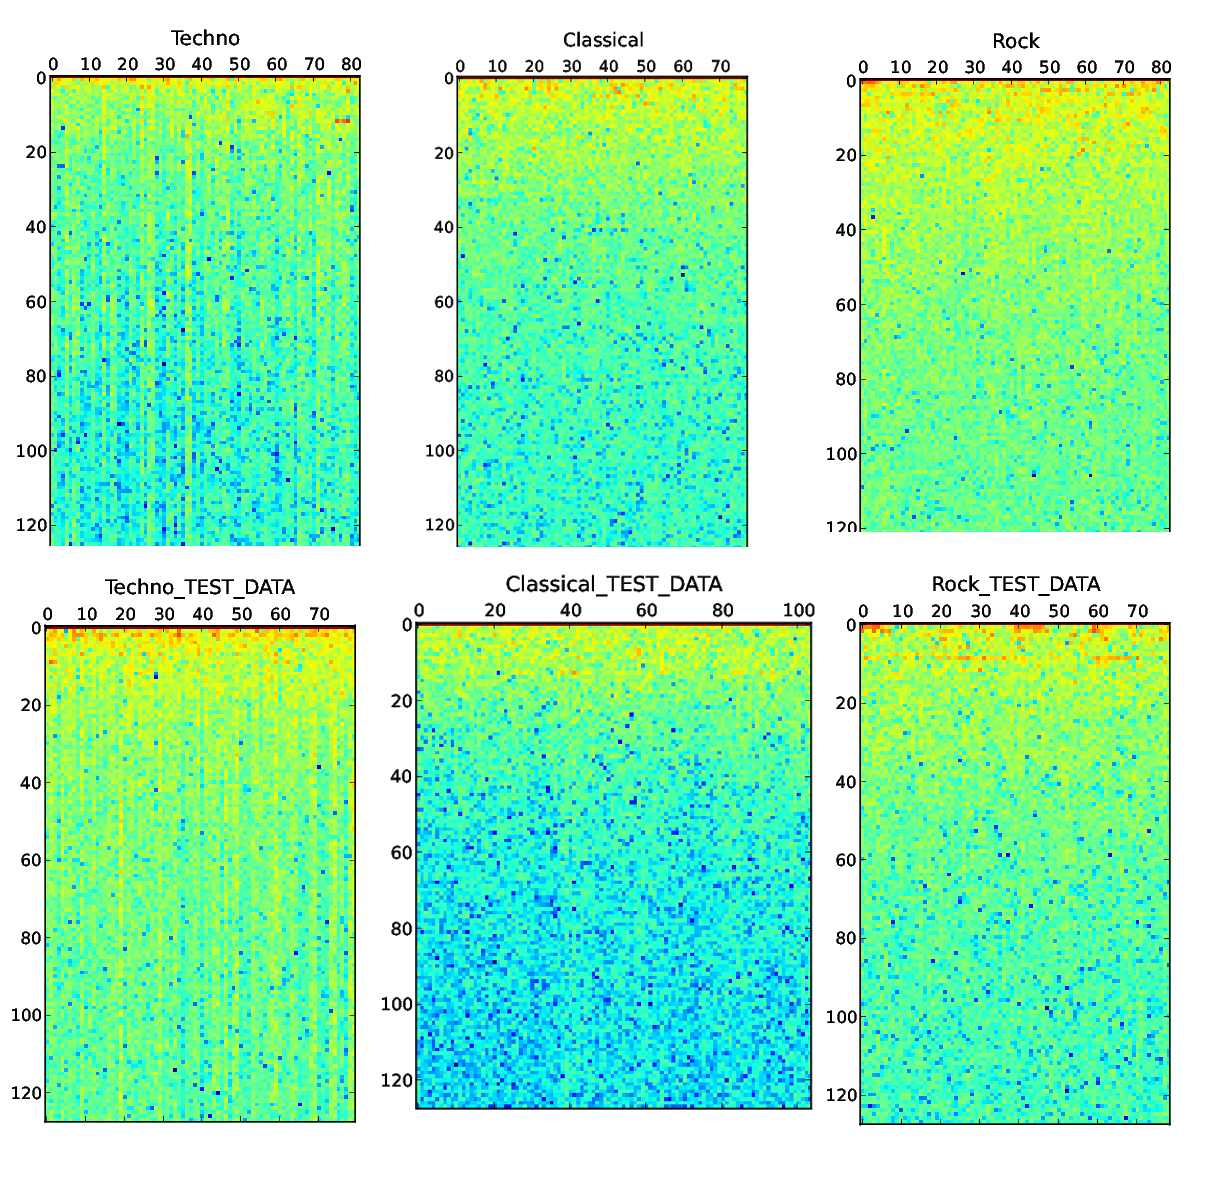
\includegraphics[scale=.5]{all_ffts.png}
\label{fig:ffts}
\end{figure}

\subsubsection{Results}
Roughly 15,000 network topologies were simulated in parallel using an eight core Intel I7 desktop computer with 16GB of RAM over the course of a week, using $\sim25$ days of total computing time.  After this extensive search of the solution space, the results in Figure ~\ref{fig:aud} were obtained. Gene layers are specified as:
\newline
$\lbrack input\_size, output\_size, overlap\_pct, \mu_s, \gamma_s, \sigma_s, \mu_r, \alpha_r, \gamma_r, \sigma_r \rbrack$.
\newline
Genomes are specified as:
\newline
$\lbrack (input\_size, output\_size),\\
 \lbrack Gene 1\rbrack \\
 \lbrack Gene 2\rbrack ...\rbrack$.
\newline

\begin{figure}[H]
\caption{New Clustering Results From Evolved Network}
\label{fig:aud}

\begin{lstlisting}
Genome:
([(128, 4),
 [128, 1, 0.66, 64, 0.04, 230, 5, 0.18, 0.53, 377],
 [  1  1, 0.60, 60, 0.12, 269, 4, 0.52, 0.43, 381],
 [  1  1, 0.64, 67, 0.25, 253, 4, 0.39, 0.31, 402]])
  
################################################################################
Results for Techno
Final Distribution Over Map Space
[ 0.349  0.506  0.     0.145]
MODE: 1
################################################################################
Results for TechnoTEST
Final Distribution Over Map Space
[ 0.4    0.325  0.     0.275]
MODE: 0
################################################################################
Results for Classical
Final Distribution Over Map Space
[ 0.103  0.051  0.     0.846]
MODE: 3
################################################################################
Results for ClassicalTEST
Final Distribution Over Map Space
[ 0.067  0.183  0.     0.75 ]
MODE: 3
################################################################################
Results for Rock
Final Distribution Over Map Space
[ 0.     0.892  0.     0.108]
MODE: 1
################################################################################
Results for RockTEST
Final Distribution Over Map Space
[ 0.  1.  0.  0.]
MODE: 1
\end{lstlisting}
\end{figure}
The engineered network for audio recognition from \cite{MLPaper} produces the results in Figure \ref{fig:audtop2}, which are superior in the separation of the data but inferior in the strength of the clustering.  This is to be expected given that the engineer in question was likely trying to obtain separation at any cost.  While the solution the genetic algorithm found was unable to fully separate Techno from Rock, the "mistake" is very narrow at 15\% of samples, and furthermore is very understandable given that Techno and Rock do share many similarities. Furthermore, the very strong separation of Classical from Rock both in and out of sample is quite promising.

\begin{figure}[H]
\caption{Old Clustering Results From Engineered Network}
\begin{lstlisting}
################################################################################
Results for Techno
Final Distribution Over Map Space
[ 0.265  0.349  0.     0.386  0.   ]
MODE: 3
################################################################################
Results for TechnoTEST
Final Distribution Over Map Space
[ 0.287  0.275  0.     0.438  0.   ]
MODE: 3
################################################################################
Results for Classical
Final Distribution Over Map Space
[ 0.526  0.154  0.     0.321  0.   ]
MODE: 0
################################################################################
Results for ClassicalTEST
Final Distribution Over Map Space
[ 0.49   0.202  0.     0.308  0.   ]
MODE: 0
################################################################################
Results for Rock
Final Distribution Over Map Space
[ 0.434  0.554  0.     0.012  0.   ]
MODE: 1
################################################################################
Results for RockTEST
Final Distribution Over Map Space
[ 0.266  0.734  0.     0.     0.   ]
MODE: 1
\end{lstlisting}
\label{fig:audtop2}
\end{figure}

\subsection{Visual Recognition of Noisy Letters}
Once the genetic algorithm had reproduced the results from the previous paper using an evolved network, the algorithm was extended to an additional domain, that of character recognition.  In this domain, 8x8 bitmap images depicting letters were shown to the networks, and consistent clustering of each letter was sought.

\subsubsection{Data}
For each letter in $\lbrace 'A', 'B', 'C', 'D' \rbrace$, the genetic algorithm uses the \texttt{setup\_letters} function from \texttt{letter\_learning.py} to generate a single "clean" copy of the letter and nine noisy copies. To investigate the robustness of the networks to noise in the visual domain, $\mathcal{N}(0,.3)$ noise was added to each letter A, B,C and D. An example of this kind of data can be seen in Figure \ref{fig:noisydataset}. 
\begin{figure}[H]
\centering
\begin{subfigure}{1.0\textwidth}
  \centering
  \includegraphics[width=1.0\linewidth]{tile_A.png}
  \caption{"A" Dataset}
\end{subfigure}

\begin{subfigure}{1.0\textwidth}
  \centering
  \includegraphics[width=1.0\linewidth]{tile_B.png}
  \caption{"B" Dataset}
\end{subfigure}

\begin{subfigure}{1.0\textwidth}
  \centering
  \includegraphics[width=1.0\linewidth]{tile_C.png}
  \caption{"C" Dataset}
\end{subfigure}

\begin{subfigure}{1.0\textwidth}
  \centering
  \includegraphics[width=1.0\linewidth]{tile_D.png}
  \caption{"D" Dataset}
\end{subfigure}%

\caption{Potential Dataset}
\label{fig:noisydataset}
\end{figure}
 
\subsubsection{Results}
After many iterations of the genetic algorithm, a number of network topologies were able to successfully cluster the clean images with their corresponding noisy images, as well as separate the four letters from each other.  For example, two networks that evolved are shown in Figure \ref{fig:letter}, where the genomes are specified as before.  After each call to \texttt{score\_letters}, the code prints out the activation vector result for each version of the letter. and finally returns the purity of all clusters.  Correct clustering is where all "A"s are clustered together, all "B"s are clustered together, etc ... and each cluster is distinct (separated).  The activation vectors are 4 vectors, and the single digit is the index of the largest value.  A purity score of 40 is a perfect score meaning that the activation vector was entirely concentrated on the index of the best matching unit, and the second genome produced a perfect score during one of the runs.  The network was simulated multiple times due to the non-determinism inherent in the system.

\begin{figure}[H]
\begin{subfigure}[b]{.5\linewidth}
\centering
\begin{lstlisting}[basicstyle=\scriptsize\ttfamily]
In [38]: g
Out[38]:
[(64, 4),
 [64,2,0.60,73,0.67,256,62,0.67,0.94, 47],
 [ 2,1,0.47,92,0.54,418,18,0.47,0.88,342],
 [ 1,1,0.22,83,0.52, 30, 4,0.52,0.22,253]]

In [39]: score_letters(g, ddata)
clean-A [3,3,3,3,3,3,3,3,3,3]
clean-B [2,2,2,2,2,2,2,2,2,2]
clean-C [1,1,1,1,1,1,1,1,1,1]
clean-D [0,0,0,0,0,0,0,0,0,0]
Out[39]: 24.116829438048846

In [40]: score_letters(g, ddata)
clean-A [0,0,0,0,0,0,0,0,0,0]
clean-B [0,0,0,0,0,0,0,0,0,0]
clean-C [2,2,2,2,2,2,2,2,2,2]
clean-D [3,3,3,3,3,3,3,3,3,3]
Out[40]: 8.7608792519449832

In [41]: score_letters(g, ddata)
clean-A [0,0,0,0,0,0,0,0,0,0]
clean-B [1,1,1,1,1,1,1,1,1,1]
clean-C [3,3,3,3,3,3,3,3,3,3]
clean-D [2,2,2,2,2,2,2,2,2,2]
Out[41]: 36.747375261437867

In [42]: score_letters(g, ddata)
clean-A [3,3,3,3,3,3,3,3,3,3]
clean-B [2,2,2,2,2,2,2,2,2,2]
clean-C [3,3,3,3,3,3,3,3,3,3]
clean-D [1,1,1,1,1,1,1,1,1,1]
Out[42]: 10.039503791155767
\end{lstlisting}
\caption{First Network Topology}
\end{subfigure}
\begin{subfigure}[b]{.5\linewidth}
\centering
\begin{lstlisting}[basicstyle=\scriptsize\ttfamily]
In [22]: x
Out[22]:
[(64, 4),
 [64,1,0.76,79,0.41,262,37,0.45,0.54,181],
 [1, 1,0.42,64,0.58,300, 4,0.52,0.24,195]]
 

In [23]: score_letters(x, ddata)
clean-A [3,3,3,3,3,3,3,3,3,3]
clean-B [0,0,0,0,0,0,2,0,0,0]
clean-C [1,1,1,1,1,1,1,1,1,1]
clean-D [2,2,2,2,2,2,2,2,2,2]
Out[23]: 37.999986356153123

In [24]: score_letters(x, ddata)
clean-A [3,3,3,3,3,3,3,3,3,3]
clean-B [2,2,2,2,2,2,2,2,2,2]
clean-C [1,1,1,1,1,1,1,1,1,1]
clean-D [0,0,0,0,0,0,0,0,0,0]
Out[24]: 40.0

In [25]: score_letters(x, ddata)
clean-A [1,1,1,1,1,1,1,1,1,1]
clean-B [0,0,0,0,0,0,1,0,0,0]
clean-C [3,1,3,3,1,3,3,3,3,3]
clean-D [2,2,2,2,2,2,2,2,2,2]
Out[25]: 33.972295936447111

In [26]: score_letters(x, ddata)
clean-A [1,1,1,1,1,1,1,1,1,1]
clean-B [3,3,3,3,3,3,3,3,3,3]
clean-C [2,2,2,2,0,2,2,2,2,2]
clean-D [0,0,0,0,0,0,0,0,0,0]
Out[26]: 37.989363926989185
\end{lstlisting}
\caption{Second Network Topology}

\end{subfigure}
\caption{Evolved Network Topologies}
\label{fig:letter}
\end{figure}

The data above shows that the networks were able to clearly distinguish letters from each other, all while being able to tolerate a significant amount of noise.

\section{Future Work \& Conclusions}
The results presented here are promising for the simulation of the lowest levels of the brain, having produced useful results in both the auditory and visual domains.  However, both data sets are fundamentally toy datasets, and real world processing would need to be able to crunch through orders of magnitude more data than 8x8 grids or 128-vectors.  In order to make this approach feasible on real world datasets, it either needs to be combined with dimensionality reductions, or it needs to be implemented on massively parallel hardware such as GPU farms.

Furthermore, additional domains such as the sensory ought be explored, although no clear reason exists that this approach would not work equally well in that domain as in the two presented in this paper.  There is also the problem that the current system only works with 1 dimensional hierarchies, when much of what 6.868 has taught is that the feedback mechanisms involved in moving beyond the basic levels of thinking and into, for example, the critics and selector models, requires extensive cross hierarchy thinking along with feedback loops.  Pursuing additional topologies that can be learned with the genetic algorithm would therefore be a very interesting direction of research.

\section{Code}
\texttt{python-hqsom} is released under the MIT license at:

\texttt{https://github.com/jolynch/python-hqsom.}


Newly written code for this project:
\begin{enumerate}
\item \texttt{genetic\_algo.py}: The genetic framework for expressing 1DHierarchies
\item \texttt{genetic\_recombination.py}: The genetic algorithm itself that actually does the search through the solution space.
\item \texttt{audio\_learning.py}: The fitness function and data preparation for the audio application.
\item \texttt{letter\_learning.py}: The fitness function and data preparation for the letter recognition.
\item \texttt{genetic\_output}: The folder containing all of the various simulated results in pickled format.
\item \texttt{som\_test.py}: The (fairly messy) runner script for all the various tests, mostly only used to generate the output for the audio networks.
\end{enumerate}

Additionally Important Code:
\begin{enumerate}
\item \texttt{som.py, rsom.py, hqsom\_audio.py} The basic implementation of the SOM, RSOM, and HQSOM algorithm along with a number of improvements over the original paper. 
\end{enumerate}

\newpage
\begin{thebibliography}{}

\bibitem{MLPaper} T. Hilk, J. Lynch \textsc{An Exploration of Hierarchical Quilted
Self-Organizing Maps}. Unpublished manuscript, 2011.

\bibitem{HQSOM} J. W. Miller and P. H. Lommel. \textsc{Biomimetic sensory abstraction using
hierarchical quilted self-organizing maps}. The Charles Stark Draper Laboratory, Inc. 555 Technology
Square, Cambridge, MA 02139-3563, USA. 2006.
\bibitem{OnIntelligence} J. Hawkins and S. Blakeslee. \textsc{On Intelligence}. Tomes Books, Holt,
New York, USA. 2002.

\bibitem{Inspiration} D. Floreano \& C. Mattiussi. \textsc{Bio-inspired artificial intelligence theories, methods, and technologies}. Cambridge, Mass: MIT Press. 2008.

\bibitem{Purity} C. Manning, P. Raghavan \& H. Schutze. \textsc{Introduction to information retrieval}. New York: Cambridge University Press. 2008
\end{thebibliography}
\newpage

\end{document}
